\chapter{Imaging 3C295 with International LOFAR}\label{section.3c295}
\minitoc
% % % % % % % % % % % % % % % % % % % % % % %
\section{Aims \& Methodology}
\pg
Our aim in this section is to create a high-resolution (0.1$''$) model of 3C295, which did not exist at LOFAR HBA frequencies when this project began. This means creating a model that will allow us to find good phase-calibration solutions for LOFAR international baselines, and thus use the international stations to create a high-resolution image of the EGS. Because we only solve for gains in the direction of 3C295, we must then estimate the impact of directional gain errors over the rest of the field.
%While we also solve for amplitude gains, we know that we will need to correct the total source flux in each frequency subband as our initial spectral model is not necessarily correct.

\pg
One major constraint in this project is that 3C295 is fully resolved at these resolutions, which makes deconvolution difficult. As such, we consistently use a $uv$-cut of $100$km throughout our imaging in this section, to limit the impact of diffuse emission (which is very hard to deconvolve properly - poor deconvolution introduces artefacts in the restored image) on our images. This choice of $uv$-cut is a compromise between removing diffuse emission in the images and providing sufficiently good conditioning to the calibration inverse problem\footnote{The more uncorrupted (i.e. flagged for RFI) visibilities are available, the better the estimation of gain solutions - see \citetads{2015MNRAS.449.2668S} for the demonstration.}. Provided that the phases of short-baseline gains do not evolve over the self-calibration procedure, then the information on spatial brightness distribution associated to these spatial fringes is not lost. 

\pg
Another constraint is that the model needs to be applicable for the full LOFAR bandwidth. We therefore select 6 sub-bands out of the total LOFAR HBA bandwidth, evenly spread throughout the bandwidth as shown in Fig. \ref{fig.freqsamp}. This approach allows us to benefit from the improved conditioning of high-frequency data (since the diffraction limit on angular resolution is proportional to frequency) throughout the LOFAR bandwidth. By starting calibration with a model extracted from a VLA observation of 3C295 with a similar angular resolution, self-calibrating over the initial 6 subbands, then self-calibrating once with 60 subbands (centred on the initial 6) and then the full bandwidth, we expect to achieve good signal-to-noise. Then, we bootstrap the model such that the spectral index of its integrated flux is compatible with \citetads{arse}.

\pg
The resulting model is expected to be reliable enough to calibrate our Groth Strip data for the full LOFAR array and the entire HBA bandwidth. Direction-dependent gains can then be used for baselines with only core and remote stations, but not those with international stations - direction-dependent effects are expected to arise in the final images due to this. Quantifying the impact of this problem is the subject of \cref{section.decorr}.

% % % % % % % % % % % % % % % % % % % % % % %
\section{Data Reduction}

\subsection{Our RIME}

\pg
As outlined in \cref{section.RIME}, calibration is the process of solving for Jones matrices, which are associated to individual antennas. Here, the only source in our model (the source that dominates, by far, over other sources in the field) is 3C295; we can thus limit ourselves to \textit{direction-independent} calibration, which is equivalent to performing direction-dependent calibration in the direction of 3C295 only. The associated RIME can be written as:
\begin{align}
\Vis_{pq}^{\nu} &= \Gjones_p^{\nu} \left( \sum_{s=3C295} \Ejones_{sp}^{\nu} \Kjones_{sp}^{\nu} \Bmatrix \left(\Kjones_{sq}^{\nu}\right)^H \left(\Ejones_{sq}^{\nu}\right)^H \right) \left(\Gjones_q^{\nu}\right)^H\\
		  &= \Gjones_p^{\nu} \Ejones_{3C295,p}^{\nu} \Bmatrix_{3C295}^{\nu} \left(\Ejones_{3C295,q}^{\nu} \Gjones_q^{\nu}\right)^H\\
		  &= \Jones_{3C295,p}^{\nu} \Bmatrix_{3C295}^{\nu} \left(\Jones_{3C295,q}^{\nu}\right)^H\label{3c295.dirin.cal}
\end{align}
where we mute the time-dependence of all terms, and explicitly model the LOFAR beam during both calibration and imaging, so as to ensure that the true sensitivity of each baseline to this out-of-phase-centre calibrator is taken into account appropriately.

\pg
What interests us here is therefore the $\Jones_{3C295,p}^{\nu}$ for all international stations $p$ and at all times and frequencies $t,\nu$. We improve conditioning by using time and frequency solution intervals of a minute and 8 subbands; at those times where this interval is too large, the quality-based weighting scheme is expected to compensate. Choosing such large intervals also helps self-calibration converge faster. We do not explicitly resort to physics-based solutions to constrain the calibration solutions: we solve for the full 8 parameters of each complex $2\times 2$ Jones matrix.



\subsection{Calibration Strategy}

\pg
We self-calibrate over the full LOFAR bandwidth so that the spectral flux distribution (i.e. where the flux of 3C295 lies at different frequencies) can be recovered in greater depth as we introduce more and more of the full bandwidth. We do not begin self-calibration with the full bandwidth, as a single pass of self-calibration with 6 subbands takes about an hour and a half, whereas it takes a full 3 days with the full bandwidth. The full bandwidth is therefore only self-calibrated on once, at the very end. We begin our self-calibration with 6 subbands, chosen across the LOFAR bandwidth, calibrated simultaneously. The chosen subbands, and their position in the total bandwidth, are shown here:
\begin{figure}[h]
\begin{floatrow}
\ffigbox{%
  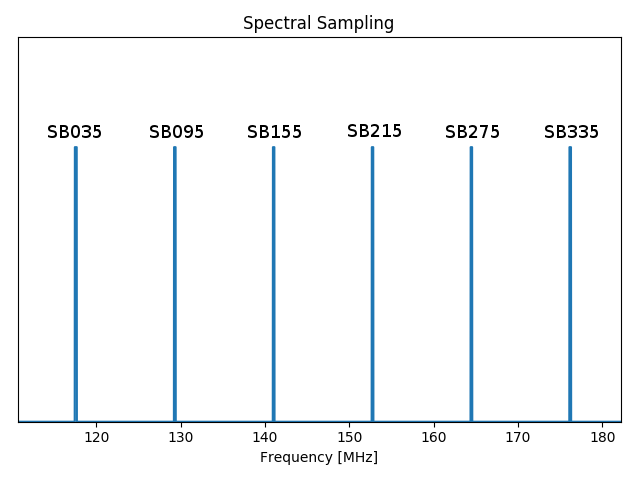
\includegraphics[width=0.5\textwidth]{images/FreqSampLabelled}
}{%
  \caption{\label{fig.freqsamp}Position of subbands chosen across full LOFAR bandwidth}%
}
\capbtabbox{%
  \begin{tabular}{|cc|} \hline
  Subband & $\nu_\mathrm{min} - \nu_\mathrm{max}$ \\ \hline
  SB035   &  117.45-117.69\\
  SB095   & 129.21-129.41\\
  SB155   & 140.93-141.12\\
  SB215   & 152.65-152.84\\
  SB275   & 164.37-164.56\\
  SB335   &  176.08-176.28 \\\hline
  \end{tabular}\vspace{1.2cm}
}{%
  \caption{Frequency bounds for the subbands chosen}%
}
\end{floatrow}
\end{figure}

\pg
Because no high-resolution models exist for 3C295 at our observing frequencies, which span quite a large bandwidth, we start by making a model from a high-resolution image taken at 8.7GHz, shown in \cref{fig.vla.3c295}. We start with a model which is as close to the expected ``true" brightness distribution because the self-calibration problem is not convex: while the calibration inverse problem itself is convex (i.e. we expect to converge towards the ``true" gains regardless of the initial conditions, given enough SNR), the degeneracy introduced by imaging in the self-calibration procedure means that one could well get stuck in a local minimum.


\pg
Because we apply a $uv$-cut of 1km when calibrating, and a $uv$-cut of 100km when imaging, we need to make sure that we do not introduce spurious structure in the core and remote station gains. Similarly, we can check the quality of our self-calibration by looking at the structure of the international station gains. Gain structure can consist of genuine atmospheric \& instrumental effects, but can also include unmodeled flux being absorbed into the gain solutions. At first, this is unavoidable: if flux is resolved by a baseline but not included in the model, then it will be absorbed into the gains. As we improve our model, we expect the gain curves to flatten and become smoother. If this happens for our international station gains, then we have a strong indication that we are in fact recovering physical signal rather than adding artefacts into our model. Similarly, we expect core and remote station gains to remain mostly static: if this is the case, then our strategy does not bias our gain solutions for these stations away from the underlying truth. 

\subsection{Testing the impact of initial model choice}

\pg
We acquire the initial calibration model by extracting features from a NASA/IPAC Extragalactic Database\footnote{\hyperref[here]{https://ned.ipac.caltech.edu/}} image of 3C295 \citepads[see][]{1991AJ....101.1623P}, shown in Fig. \ref{fig.vla.3c295}. This feature extraction is carried out using PyBDSM \citepads{2015ascl.soft02007M}, changing all extracted Gaussians into points\footnote{This practice ensures that wrongly-estimated Gaussians do not end up introducing unphysical bias during calibration.}.
\begin{figure}[h]
\includegraphics[width=0.8\linewidth]{images/{3C_295_I_8.7GHz_lbs2003.fits}.png}
\caption{\label{fig.vla.3c295}VLA observation of 3C295 at 8.7 GHz. Pixel size is $0.2''$.}
\end{figure}
% command: python ~/Scripts/PngCutoutFromFits.py --filename 3C_295_I_8.7GHz_lbs2003.fits --RA 14:09:33.418 --Dec 52:26:13 --size .12 --vmin -0.5 --vmax 4 --invert

\pg
A good initial test of our hypothesis that we can start from a ``good enough" point to reach a global minimum is to self-calibrate on a two-point model. We perform this test, keeping only the two brightest pixels of the model shown above to test whether we converge to the same structure. The result is shown as an overlay in \cref{fig.sc.2pt}: as we can see, we recover the same structure as the full VLA model. We appear to have introduced a small astrometric error, however: this is likely an indicator that using only the peak flux, rather than the full distribution, will bias the ``centre of flux" away from its true position -- hence introducing an astrometric shift. We therefore start from the full model for our ``proper" self-calibration procedure.
\begin{figure}[h]
\includegraphics[width=0.8\linewidth]{images/{3C_295_I_8.7GHz_lbs2003.J2000.fits2ptmodel}.png}
\caption{\label{fig.sc.2pt} Overlay of the model resulting from a self-calibration process starting from a two-point model. The overlays rise exponentially, from the $5\sigma$ level to the maximum pixel value in the image. This image is very similar to the LOFAR image made with a single pass of calibration using the full VLA model.}
\end{figure}

\pg
The only exhaustive method to test our hypothesis would be to perform a full Monte Carlo analysis, testing every possible flux distribution for every pixel at every frequency to ensure that we do, in fact, find the model and gains which give the global minimum fit, rather than a local minimum fit. This would be extremely time-consuming, however, and falls outside the scope of this work. We therefore simply try to start as close as possible to where we expect the global minimum to fall, using the full VLA image as a starting model.

\subsection{Frequency-dependent Scale Error}

\pg
We begin by using a simple spectral index of $\alpha=-0.8$, which is typical of synchrotron sources at these frequencies. It is not strictly correct, but gives a good first-order approximation of the integrated flux of 3C295 as a function of frequency, which is shown in \cref{fig.3c295.intflux}
\begin{figure}[h]
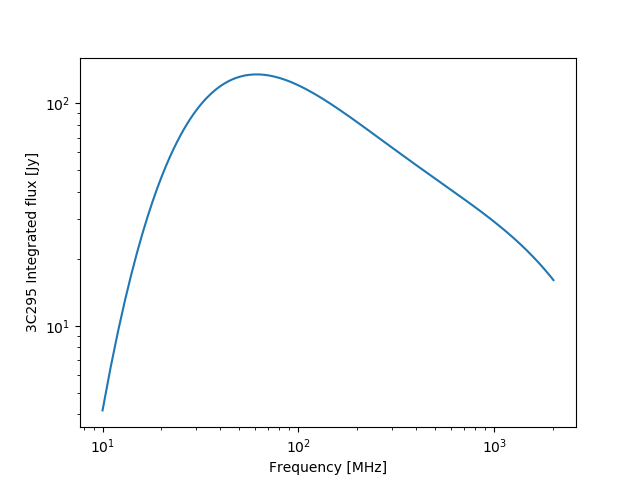
\includegraphics[width=0.8\linewidth]{images/3C295-intflux.png}
\caption{\label{fig.3c295.intflux} Integrated flux of 3C295 as a function of frequency, as fitted by \citepads{arse}.}
\end{figure}


In so doing, we introduce a frequency-dependent error factor in our gain solutions:
\begin{align}
\hatJones_{3C295,p}^{\nu} &\approx \sqrt{\alpha_\nu} \Jones_{3C295,p}^{\nu}
\end{align}
where $\hatJones_{3C295,p}^{\nu}$ is our estimation of the Jones matrix $\Jones_{3C295,p}^{\nu}$ for time $t$ and frequency $\nu$. $\alpha_\nu$ is a smoothly-varying function of frequency alone. This then introduces a frequency-dependent error factor $1/\sqrt{\alpha_\nu}$ in our visibilities and therefore in our images. This factor is a constant for all visibilities at a given frequency.

\pg
Because we solve for the full Jones matrix, we cannot apply phase-only corrections\footnote{Indeed, what is the phase of a $2\times2$ matrix of complex numbers?} over multiple self-calibration rounds, as is standard practice. Over self-calibration rounds, we expect that $\alpha$ will change, but that it will remain smooth in frequency. The integrated flux of 3C295 over different passes of self-calibration is shown in \cref{fig.SC.ampfluct}: as this figure shows, the model amplitude can diverge significantly over the self-calibration process. %, sometimes even moving closer to the inital integrated flux, but often moving farther. 

% images:
% IMAGES/3c295.fromVLA.6sb.withbeam.pass[1-5].int.model.fits IMAGES/3c295.fromVLA.60sb.withbeam.pass[1-3].int.model.fits IMAGES/MSlist.fullBW.LOBOS6.MSlist.fullBW.txt.uniform.int.model.fits
% script: /home/offler/plotSCamp.py
\begin{figure}[h!]
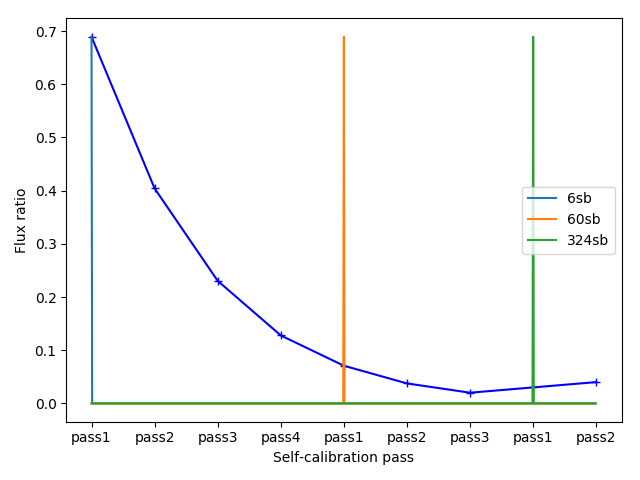
\includegraphics[width=0.8\linewidth]{images/AmpFluct.png}
\caption{\label{fig.SC.ampfluct} Amplitude fluctuation of the models resulting from self-calibration iterations, expressed as a ratio of the model's integrated flux divided by the Scaife \& Healde integrated flux model at the appropriate frequency. Note that the integrated model flux for 324sb-pass1 (the penultimate data point in this plot) was lost to a careless command: the value shown here is just the average of the two neighbouring values.}
\end{figure}

\pg
Because $\alpha$ is smooth in frequency, we can apply a frequency-dependent amplitude correction (i.e. ``bootstrap") by relying on the work of Scaife \& Heald \citep[see][]{arse}. This correction will be done in the imaging plane, since $alpha$ is a function of $uv$-position (but not sky position). This is, again, because 3C295 does not lie at phase centre: if it did, the correction could be done equivalently in visibility or image space. By performing it in the image-plane, we rid ourselves of the $uv$-dependence. The resulting signal-to-noise improvement is shown in \cref{fig.SCrms}. It is calculated on the bootstrapped residual images resulting from each round of the self-calibration process - as such, the only thing that changes is the noise, since the signal is corrected to be the appropriate constant As we can see, the noise falls nicely with self-calibration passes. Tragically, the results from the first full-bandwidth calibration run with the 60-subband model were lost before this plot could be made, and so only the results from the second full-bandwidth self-calibration pass remain. We can see that it is a small improvement over the 60-subband model. 
\begin{figure}[h!]
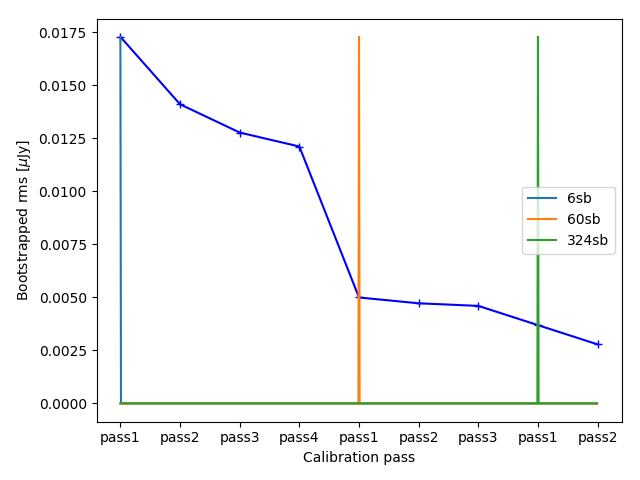
\includegraphics[width=0.8\linewidth]{images/SCrms.png}
\caption{\label{fig.SCrms} Bootstrapped residual RMS for each calibration pass. Note that the data for 324sb-pass1 (the penultimate data in this plot) were lost to a careless command: the value shown here is just the average of the two neighbouring values.}
\end{figure}

\pg
The large decrease (factor of $\sim2$)in RMS between the last 6-subband residual image and the first 60-subband residual image in \cref{fig.SCrms} is significant: we would expect a similar jump when going from 60 to 324 subbands. The fact that we do not is a strong indicator that we are digging into the limits of what our strategy can achieve by the end of the second full-bandwidth self-calibration pass: we are stuck in a local minimum. This is likely due to the fact that our initial sky model (and all subsequent models) only include 3C295: the fact that all the other sources in the primary beam are not included in the model is bound to introduce bias our gain solutions and artefacts in our images. 

\pg
We want good phase and amplitude gain estimates without concern for the overall scaling factor: this means that we want to find the correct brightness distribution at a given frequency, knowing that the overall scaling factor will be wrong, and correcting the images accordingly afterwards. 


\subsection{Examining gain solutions}


\pg
Let us begin by checking whether our core and remote station gains change over time due to our self-calibration procedure. Here, we look at the gains of SB155, on which we solved for gain solutions using our initial and final models. This subband was included in the 60-subband self-calibration step, but not the 6-subband self-calibration step.
\begin{figure}[h!]
\begin{subfigure}{.9\textwidth}
\includegraphics[width=\linewidth]{images/{SB155.CS005HBA0.firstpass}.png}
\caption{\label{fig.sb155.gains.cs201.before} CS005, first calibration}
\end{subfigure}
\begin{subfigure}{.9\textwidth}
\includegraphics[width=\linewidth]{images/{SB155.CS005HBA0.lastpass}.png}
\caption{\label{fig.sb155.gains.cs201.after} CS005, last calibration}
\end{subfigure}
\begin{subfigure}{.9\textwidth}
\includegraphics[width=\linewidth]{images/{SB155.RS305HBA.firstpass}.png}
\caption{\label{fig.sb155.gains.RS305.before} RS305, first calibration}
\end{subfigure}
\begin{subfigure}{.9\textwidth}
\includegraphics[width=\linewidth]{images/{SB155.RS305HBA.lastpass}.png}
\caption{\label{fig.sb155.gains.RS305.afer} RS305, last calibration}
\end{subfigure}
\caption{\label{fig.sb155.gains.CR} Gain amplitude \& phase for CS201 of SB155}
\end{figure}

\pg
As we can see from \cref{fig.sb155.gains.CR}, there is little change in amplitude structure between the first pass of calibration (with the model extracted from \cref{fig.vla.3c295}) and the last pass of calibration (after the successive self-calibration passes). Similarly, there is little apparent change in phase structure (note that the phase wraps from $-\pi$ to $\pi$). It is important to note, however, that there is a difference in the \textit{level} of the amplitude curve: in the first pass of calibration, the average amplitude value is generally higher than in the last pass of calibration. This is expected behaviour, as there is less diffuse emission in the $uv$-cut imaging model of 3C295 than in the initial calibration model. This is equivalent to applying a choice of weighting scheme which down-weighs diffuse emission (i.e. a form of uniform weighting).

\pg
As for the international station gains, they are shown below for three of the seven international stations used for our observation, in \cref{fig.sb155.gains.de602,fig.sb155.gains.se607,fig.sb155.gains.uk608}. We show only one of the four German stations. As we can see, while structure very clearly remains in some of these amplitude curves (notable in the last two hours, e.g. \cref{fig.sb155.gains.DE602.after}), some of the structure disappears from these amplitude curves. It should be noted that the last two hours of the observation are generally much noisier than the first 6; the last quarter of these plots show this. Quality-based weighting schemes compensate for this effect, and minimise the associated image deterioration. Note that the phase wraps extremely fast in the international station gain plots: this is because phase is calculated relative to CS001HBA0, the first antenna in our array. Because the international stations are much farther away from this core station than other core or remote stations are, we expect the associated phase solutions to wrap faster.
\begin{figure}[h!]
\begin{subfigure}{.9\linewidth}
\includegraphics[width=\linewidth]{images/{SB155.DE602HBA.firstpass}.png}
\caption{\label{fig.sb155.gains.DE602.before} DE602, first calibration}
\end{subfigure}
\begin{subfigure}{.9\linewidth}
\includegraphics[width=\linewidth]{images/{SB155.DE602HBA.lastpass}.png}
\caption{\label{fig.sb155.gains.DE602.after} DE602, last calibration}
\end{subfigure}
\caption{\label{fig.sb155.gains.de602} Gain amplitude \& phase for DE602 of SB155}
\end{figure}

\begin{figure}[h!]
\begin{subfigure}{.9\textwidth}
\includegraphics[width=\linewidth]{images/{SB155.SE607HBA.firstpass}.png}
\caption{\label{fig.sb155.gains.SE607.before} SE607, first calibration}
\end{subfigure}
\begin{subfigure}{.9\textwidth}
\includegraphics[width=\linewidth]{images/{SB155.SE607HBA.lastpass}.png}
\caption{\label{fig.sb155.gains.SE607.after} SE607, last calibration}
\end{subfigure}
\caption{\label{fig.sb155.gains.se607} Gain amplitude \& phase for SE607, an international stations of SB155}
\end{figure}

\begin{figure}[h!]
\begin{subfigure}{.9\textwidth}
\includegraphics[width=\linewidth]{images/{SB155.UK608HBA.firstpass}.png}
\caption{\label{fig.sb155.gains.UK608.before} UK608, first calibration}
\end{subfigure}
\begin{subfigure}{.9\textwidth}
\includegraphics[width=\linewidth]{images/{SB155.UK608HBA.lastpass}.png}
\caption{\label{fig.sb155.gains.UK608.after} UK608, last calibration}
\end{subfigure}
\caption{\label{fig.sb155.gains.uk608} Gain amplitude \& phase for UK608HBA, an international stations of SB155}
\end{figure}

\pg
So far, we have shown the gain solutions for one subband, out of a total of 324 used subbands. The spectral behaviour of the amplitude and phase solutions can give us insight into whether we are absorbing true flux or calibration artefacts into our model: if our calibration model becomes more accurate to the true underlying flux, we expect e.g. the phase of core station calibration solutions to remain the same (as we are improving high-resolution details of our model) while our international station calibration solutions would become flatter in amplitude. Similarly, we expect to see large-scale frequency-dependent behaviour in the phase solutions of international stations, with smaller fluctuations around this behaviour: the effect of differential TEC, ionospheric turbulence, etc. Indeed, while the core stations (and, to a lesser extent, the remote stations) can be approximated as having the ``same ionosphere" above them, this is not the case for international stations: this is a major source of the difficulties in calibrating these stations. As such, for international stations, we expect to see complex structure in the phase gain solutions, characteristic of the differences between the local atmosphere above the core and the international stations. For core stations, we only expect to see structure characteristic of scintillation (regular stripes with no frequency-dependent structure) in the phase gain solutions. 

\pg
\cref{fig.fullBW.CS005,fig.fullBW.CS201HBA0} show the gain solution phases and amplitudes for all times and frequencies in our observation. Some patches of the plot are empty (horizontal red bands): this is because some subbands had very poor data, and their use in self-calibration corrupted the final image. They are more numerous for the first calibration pass than the last, as the solutions were not sought for some cases.

\begin{figure}[h!]
\begin{subfigure}{.9\textwidth}
\includegraphics[width=\linewidth]{images/{CS005HBA0.firstpass.fullBW}.png}
\caption{\label{fig.fullBW.gains.CS005.before} CS005HBA0, first calibration, full bandwidth}
\end{subfigure}
\begin{subfigure}{.9\textwidth}
\includegraphics[width=\linewidth]{images/{CS005HBA0.lastpass.fullBW}.png}
\caption{\label{fig.fullBW.gains.CS005.after} CS005HBA0, last calibration, full bandwidth}
\end{subfigure}
\caption{\label{fig.fullBW.CS005} Plots showing the amplitude and phase solutions for CS005HBA0 at the start and end of self-calibration, respectively. The black areas correspond to regions which were not used for that pass of calibration due to poor data.}
\end{figure}

\begin{figure}[h!]
\begin{subfigure}{.9\textwidth}
\includegraphics[width=\linewidth]{images/{CS201HBA0.firstpass.fullBW}.png}
\caption{\label{fig.fullBW.CS201HBA0.before} CS201HBA0, first calibration, full bandwidth}
\end{subfigure}
\begin{subfigure}{.9\textwidth}
\includegraphics[width=\linewidth]{images/{CS005HBA0.lastpass.fullBW}.png}
\caption{\label{fig.fullBW.CS201HBA0.after} CS201HBA0, last calibration, full bandwidth}
\end{subfigure}
\caption{\label{fig.fullBW.CS201HBA0} Plots showing the amplitude and phase solutions for CS201HBA0 at the start and end of self-calibration, respectively. The black areas correspond to regions which were not used for that pass of calibration due to poor data.}
\end{figure}

\pg
As we can see, the behaviour of both phase and amplitude gains remains much the same for core stations, before and after self-calibration. This is a good sign: it means that we do not lose the large-scale structure in our observation as we self-calibrate. We see in \cref{fig.fullBW.RS305HBA} that remote stations have much more phase structure as a function of frequency. This structure shows that the ionosphere above the remote Dutch stations is different from that above the core stations: this is an expected result. The fact that the structure does not change significantly before and after the self-calibration run could indicate that the remote station gains, like the core stations gains, do not absorb true flux into their gain solutions during the self-calibration process. It can thus be taken as a sign that our self-calibration is trustworthy for these stations.
\begin{figure}[h!]
\begin{subfigure}{.9\textwidth}
\includegraphics[width=\linewidth]{images/{RS305HBA.firstpass.fullBW}.png}
\caption{\label{fig.fullBW.RS305HBA.before} RS305HBA, first calibration, full bandwidth}
\end{subfigure}
\begin{subfigure}{.9\textwidth}
\includegraphics[width=\linewidth]{images/{RS305HBA.lastpass.fullBW}.png}
\caption{\label{fig.fullBW.RS305HBA.after} RS305HBA, last calibration, full bandwidth}
\end{subfigure}
\caption{\label{fig.fullBW.RS305HBA} Plots showing the amplitude and phase solutions for RS305HBA at the start and end of self-calibration, respectively. The black areas correspond to regions which were not used for that pass of calibration due to poor data.}
\end{figure}

\pg
Finally, we examine the gain solutions for international stations. This is where we expect to see the most significant amplitude and phase structure, but also where we expect gain structure to change between the start and end of the self-calibration process. If this is the case, it would mean that the unmodeled astrophysical signal that is initially absorbed into international station gain solutions is introduced into the model over multiple iterations. Notably, we expect a big change in amplitude solutions; phase solutions are harder to read, as we expect the ionosphere to be drastically different between core and international stations. As such, they will include both true phase structure and the contribution of unmodeled flux.

\begin{figure}[h!]
\begin{subfigure}{.9\textwidth}
\includegraphics[width=\linewidth]{images/{DE601HBA.firstpass.fullBW}.png}
\caption{\label{fig.fullBW.DE601HBA.before} DE601HBA, first calibration, full bandwidth}
\end{subfigure}
\begin{subfigure}{.9\textwidth}
\includegraphics[width=\linewidth]{images/{DE601HBA.lastpass.fullBW}.png}
\caption{\label{fig.fullBW.DE601HBA.after} DE601HBA, last calibration, full bandwidth}
\end{subfigure}
\caption{\label{fig.fullBW.DE601HBA} Plots showing the amplitude and phase solutions for DE601HBA at the start and end of self-calibration, respectively. The black areas correspond to regions which were not used for that pass of calibration due to poor data.}
\end{figure}

\begin{figure}[h!]
\begin{subfigure}{.9\textwidth}
\includegraphics[width=\linewidth]{images/{DE602HBA.firstpass.fullBW}.png}
\caption{\label{fig.fullBW.DE602HBA.before} DE602HBA, first calibration, full bandwidth}
\end{subfigure}
\begin{subfigure}{.9\textwidth}
\includegraphics[width=\linewidth]{images/{DE602HBA.lastpass.fullBW}.png}
\caption{\label{fig.fullBW.DE602HBA.after} DE602HBA, last calibration, full bandwidth}
\end{subfigure}
\caption{\label{fig.fullBW.DE602HBA} Plots showing the amplitude and phase solutions for DE602HBA at the start and end of self-calibration, respectively. The black areas correspond to regions which were not used for that pass of calibration due to poor data.}
\end{figure}

\begin{figure}[h!]
\begin{subfigure}{.9\textwidth}
\includegraphics[width=\linewidth]{images/{DE603HBA.firstpass.fullBW}.png}
\caption{\label{fig.fullBW.DE603HBA.before} DE603HBA, first calibration, full bandwidth}
\end{subfigure}
\begin{subfigure}{.9\textwidth}
\includegraphics[width=\linewidth]{images/{DE603HBA.lastpass.fullBW}.png}
\caption{\label{fig.fullBW.DE603HBA.after} DE603HBA, last calibration, full bandwidth}
\end{subfigure}
\caption{\label{fig.fullBW.DE603HBA} Plots showing the amplitude and phase solutions for DE603HBA at the start and end of self-calibration, respectively. The black areas correspond to regions which were not used for that pass of calibration due to poor data.}
\end{figure}

\pg
We see that some of the structure in the amplitude gains shown in \cref{fig.fullBW.DE601HBA} goes away over the course of self-calibration, though one of the two arcs present in the plot appears to decrease in amplitude. For \cref{fig.fullBW.DE602HBA}, we see that the pattern in the amplitude plot clearly changes - the fact that the pattern in \cref{fig.fullBW.DE602HBA.before} does not appear to be either dispersion or scintillation pattern would indicate that it consists of unmodeled flux. While some structure remains in the last 2 hours and low frequencies for this antenna's gain solution amplitudes, the last 2 hours of the observation are generally poor compared to the first six: we expect that the quality-based weighting scheme will minimise the impact of these poor calibration solutions on the final images. In \cref{fig.fullBW.DE603HBA}, we see that the self-calibration process was clearly less effective than it was for DE602HBA: while some of the structure was minimised (in the first two hours particularly: we go from the peculiar ``ellipse" pattern to something which looks more like scintillation), a lot clearly remains. Our self-calibration process could therefore likely be taken further. However, in our last step, we use 324 out of the full 366 subbands (leaving some out due to poor quality); a single round of self-calibration with this full dataset takes 5000 minutes on the best computing cluster available for this work. Because a single round of self-calibration would, at this point, take as much time as imaging a portion of the EGS due to computational constraints, we treat the self-calibration process as ``having converged" at this point: while it could be yet improved, we have reached a signal-to-noise of 2.78mJy. 


\clearpage
% % % % % % % % % % % % % % % % % % % % % % %
\section{Overlays \& Spectral Analaysis}

\pg
The final, high-resolution, multi-frequency, bootstrapped model of 3C295 - which gives a spectral index for each pixel in the model - is shown in \cref{fig.3c295.final}. An overlay of this model is shown in \cref{fig.3c295.final.overlay}. The brightness distribution seems to have largely stayed within the bounds of the initial model for the southern lobe, but to have shifted eastwards for the northern lobe. We see that artefacts remain in the field, but this is not the case at all frequencies, as shown in \cref{fig.3c295.spectral.overlays}: three of the six slices seem to be much better-calibrated than their peers. It should be noted that we both maximise the presence of calibration artefacts \textit{and} minimise the contribution of diffuse emission through our choices of weighting scheme and imaging $uv$-cut, respectively.

\begin{figure}[h]
\includegraphics[width=0.9\linewidth]{images/{MSlist.fullBW.LOBOS6.MSlist.fullBW.txt.uniform.int.convmodel.bootstrap.fits}.png}
\caption{\label{fig.3c295.final} Final model of 3C295.}
\end{figure}

\begin{figure}[h]
\includegraphics[width=0.9\linewidth]{images/{3C_295_I_8.7GHz_lbs2003.J2000.fits.overlay}.png}
\caption{\label{fig.3c295.final.overlay} Overlay of final model of 3C295 on initial VLA model. This final model is made by adding individual contributions from the spectral slices shown in \cref{fig.3c295.spectral.overlays}.}
\end{figure}
% python ~/Scripts/PngCutoutFromFits.py --filename 3C_295_I_8.7GHz_lbs2003.J2000.fits --RA 14:11:20.6 --Dec 52:12:09.0 --size .1 --invert -v --overlaymin 10 --nlevels 200 --vmin 0.06 --vmax 2 --overlay IMAGES/MSlist.fullBW.LOBOS6.MSlist.fullBW.txt.uniform.int.restored.bootstrap.fits
\pg
By inspecting individual spectral slices of our multi-spectral model in \cref{fig.3c295.spectral.overlays}, we can see that the presence of calibration artefacts is not the same at all frequencies. We see a lot of artefacts remain for the slice at 176.17 MHz in particular, and the slice at 140.428 MHz to a lesser extent. Note that the overlay values rise exponentially. The maximum pixel value  in the image is $\sim$20 Jy, while the noise in the corner of the image is $\sim$2mJy. We achieve a relatively decent dynamic range (DR=10000, which is a factor of 100 lower than what is achievable with self-cal on VLA, WSRT data). We note that the dynamic range here is lower than could be expected for this data. This could be due, among other things, to our choices of $uv$-cut and imaging weights, both of which ``artificially" increase the rms in the image (but are necessary to improve image deconvolution for such a diffuse source. However, considering the still-large presence of artefacts near 3C295, it is likely that we ended up in a local minimum by not modeling all the sources in the field.


\begin{figure}[h!]
\begin{subfigure}{.49\textwidth}
\includegraphics[width=\linewidth]{images/{3C_295_I_8.7GHz_lbs2003.J2000.fitsfreq0}.png}
\caption{\label{fig.3c.model.freq0} Overlay of our model of 3C295 at 116.6 MHz over our initial VLA model.}
\end{subfigure}
\begin{subfigure}{.49\textwidth}
\includegraphics[width=\linewidth]{images/{3C_295_I_8.7GHz_lbs2003.J2000.fitsfreq1}.png}
\caption{\label{fig.3c.model.freq1} Overlay of our model of 3C295 at 128.514 MHz over our initial VLA model.}
\end{subfigure}
\begin{subfigure}{.49\textwidth}
\includegraphics[width=\linewidth]{images/{3C_295_I_8.7GHz_lbs2003.J2000.fitsfreq2}.png}
\caption{\label{fig.3c.model.freq2} Overlay of our model of 3C295 at 140.428 MHz over our initial VLA model.}
\end{subfigure}
\begin{subfigure}{.49\textwidth}
\includegraphics[width=\linewidth]{images/{3C_295_I_8.7GHz_lbs2003.J2000.fitsfreq3}.png}
\caption{\label{fig.3c.model.freq3} Overlay of our model of 3C295 at 152.342 MHz over our initial VLA model.}
\end{subfigure}
\begin{subfigure}{.49\textwidth}
\includegraphics[width=\linewidth]{images/{3C_295_I_8.7GHz_lbs2003.J2000.fitsfreq4}.png}
\caption{\label{fig.3c.model.freq4} Overlay of our model of 3C295 at 164.256 MHz over our initial VLA model.}
\end{subfigure}
\begin{subfigure}{.49\textwidth}
\includegraphics[width=\linewidth]{images/{3C_295_I_8.7GHz_lbs2003.J2000.fitsfreq5}.png}
\caption{\label{fig.3c.model.freq5} Overlay of our model of 3C295 at 176.17 MHz over our initial VLA model.}
\end{subfigure}
\caption{\label{fig.3c295.spectral.overlays} Overlays of individual slices of our spectral model of 3C295 over our initial calibration model. The overlays start at 1500$\sigma$, and are shown with increments of 1500$\sigma$.}
\end{figure}

\pg
It is interesting to note that the rms value in each individual slice is comparable to the rms value in the ``collapsed" model (average of all slices), where we would expect it would decrease by a factor $\sim\sqrt{6}$ (i.e. about 2.5). The fact that this does not occur is a strong indication that we are in a regime where we are dominated by calibration artefacts, and that the rms is therefore not truly thermal. It is also an indication that we could likely improve the self-calibration strategy: this behaviour could be due to too small a deconvolution mask, for example.

\pg
Note that each individual pixel of our model has its own spectral index: after bootstrapping the model, we therefore have a full spectral model of 3C295 across the LOFAR HBA bandwidth, with an integrated flux compatible with the literature and a spectral brightness distribution determined by our observation. This model can be used to perform direction-independent calibration of all future observations of the EGS.

\clearpage
\section{Discussion}

\pg
The plots of pre-self-calibration gain amplitude and phases as a function of frequency are a strong indicator that the gain structure due to unmodeled flux is dominated by a strong, bright source (ring-like structure in e.g. \cref{fig.fullBW.DE603HBA}). However, the remaining presence of diffuse ring-like structure, even after the self-calibration process, for the international station gain plots is also a strong indicator that we do not recover all of the true sky brightness distribution in the model, as some of the flux is still clearly absorbed into the gains. The most straightforward way to improve on this would be to repeat the procedure while including a full low-resolution sky model: while 3C295 is by far the brightest source in the field at a recorded $\sim$86.9 Jy in the catalog of the sources in our wide-field image (\cref{table.egs.sources}), it is far from the only contributor (the net flux in the field, according to that same catalog, is 531.1 Jy). Since calibration artefacts are introduced by both incomplete sky model and poor calibration inverse problem conditioning, improving one of these two conditions would likely result in a net improvement of the model. % It was a mistake not to have done so from the very beginning. %, and one which I would not repeat if this was to be redone.

\pg
Because of time/computational constraints, we used calibration solution intervals of 8 channels and 1 minute in time and frequency respectively. Given the brightness of 3C295, this was clearly not justified on the basis of signal-to-noise; it did, however, mean that a single pass of self-calibration on one subband took 10 minutes rather than an hour and a half (factor of 9 improvement in time). With the advent of new tools like cubical \citepads{2018MNRAS.tmp.1165K,2018ascl.soft05031K}, a much faster direction-independent implementation of the algorithm used for killMS\footnote{In the context of this work, it would literally be an equivalent but faster implementation of exactly the same algorithm.} which was in development throughout my PhD, it is likely possible to dramatically speed the calibration part of the self-calibration loop (the imaging time constraint would dominate as more subbands are added). Because of the use of quality-based weighting schemes, it is unlikely that a dramatic improvement would be seen when self-calibrating over a few subbands, as the relative contribution of poorly-calibrated visibilities would be down-weighted by the quality-based weighting scheme: as more and more data is added, however, the relative contribution of the artefacts introduced by the choice of calibration intervals would likely begin to overcome the purely thermal noise in the images, which is expected to decrease as more data is added.% in the well-calibrated visibilities, even when down-weighted.

\pg
All the same, this project served as a useful exercise in both developing a good working methodology and in testing calibration strategies for international LOFAR datasets. Much of the development which went into this project and led to no directly useful results still proved an extremely helpful context in which to understand how to improve the LOFAR pipeline. In particular, gain smoothing has shown promising result on LOTSS images, but was not used in this project because of the full-Jones solutions: properly implementing this smoothing in polarisation could provide the kind of regularisation that our gain solutions need.

%
%\pg
%The last significant error which I see in the strategy followed here - error in the sense that, should I do the same work again, I would likely do this differently - is a methodological one: knowing what I learned over the course of this project, I would likely have been able to identify and prevent time-consuming digressions in my work, which led to time-consuming errors needing to be corrected. It took me over a year to begin to rigorously follow a strategy, even if it may be flawed: trying to hand-correct individual aspects of the strategy on the fly (and with so many aspects being arbitrary, inevitably losing track of where I was at points) was a flaw which took me a while to overcome. % It is difficult to be satisfied with a ``good enough" result (after all, the person reducing the data knows all too well just how poor ``good enough" can be), but it is necessary. While I do not feel that the results presented here truly are ``good enough", I am confident that the methodology used to achieve them is sound.
%
%\pg
%The last section of this thesis shows work done to test the quality of our international station gains (or, equivalently, of our model of 3C295). 
%
%
%
